\section{Frequency Domain Filtering}
\subsection{Fourier-Transform}
Octave wouldn't let me save the plots. It complained about a library that wasn't in the package manager not being available.
I took screenshots and have included those. Enjoy.

\begin{figure}[H]
    \begin{subfigure}{0.5\textwidth}
        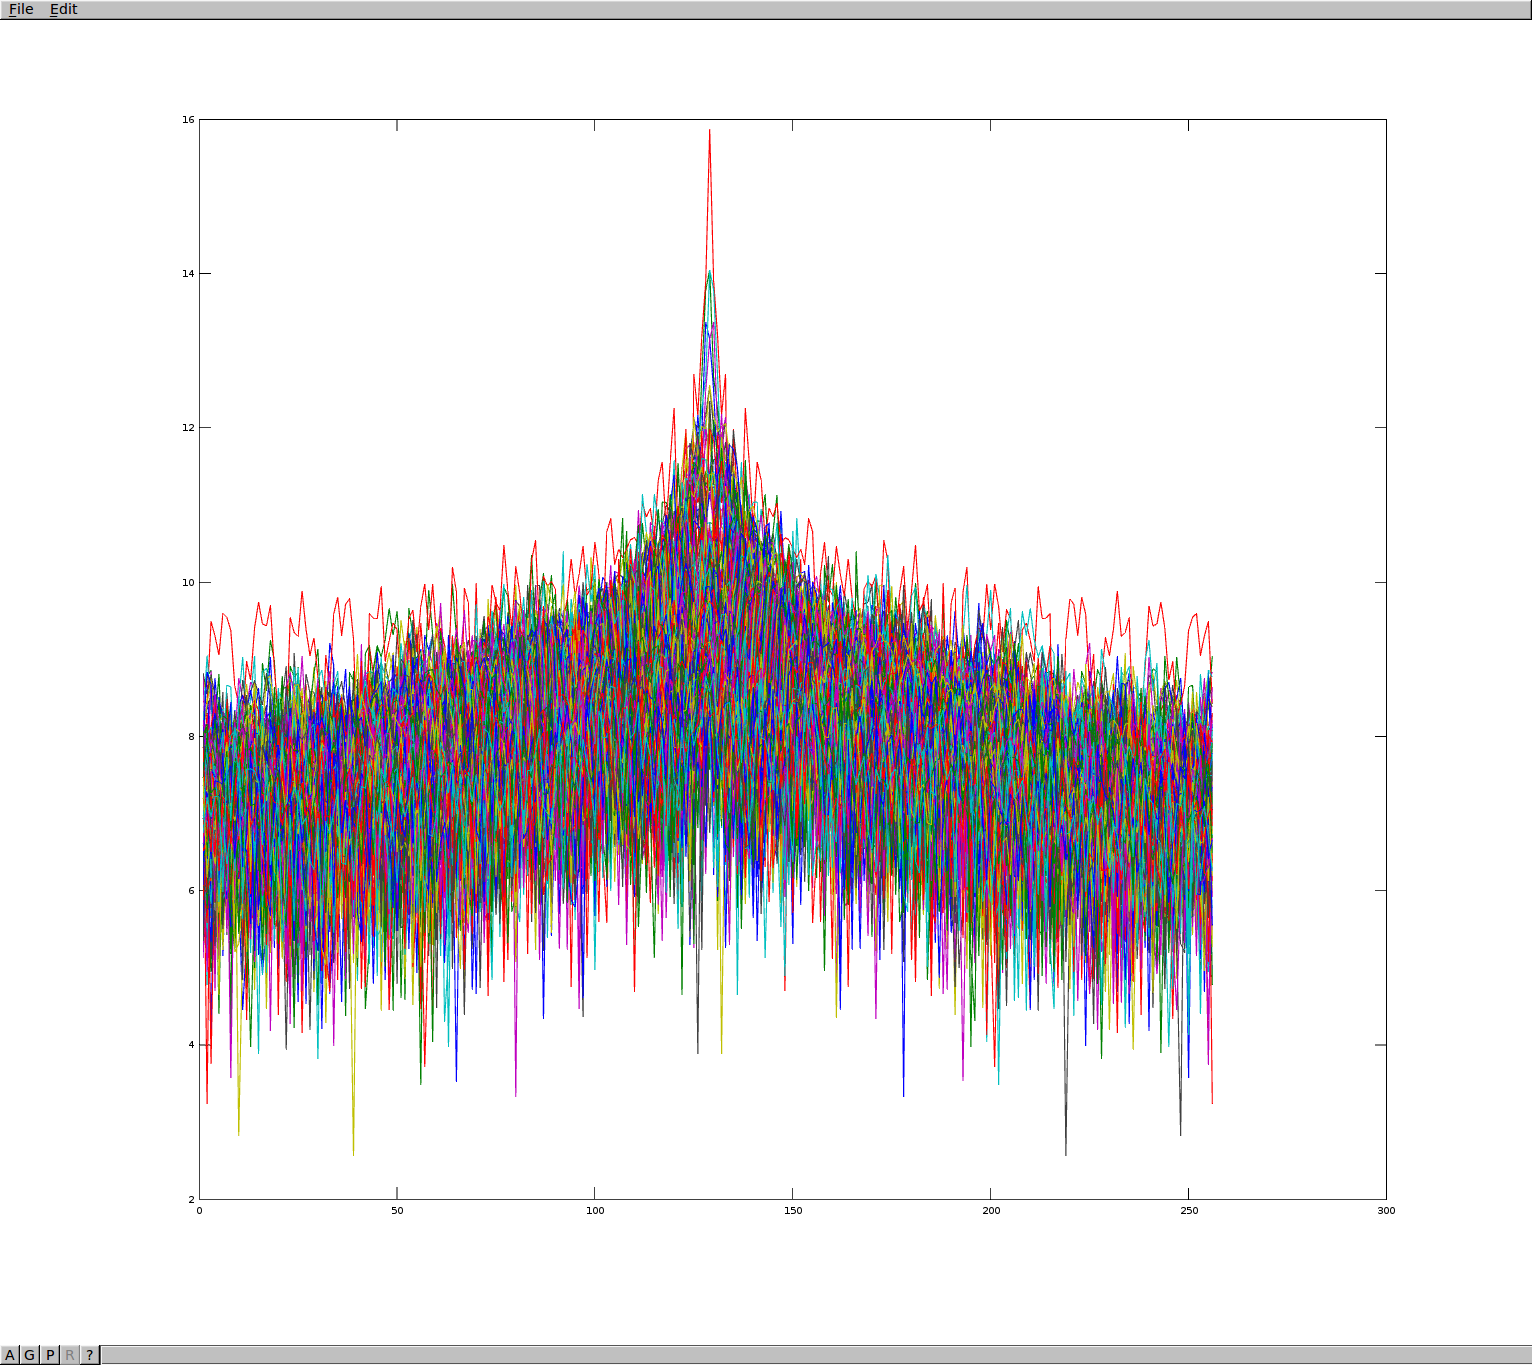
\includegraphics[width=\textwidth]{../code/3_out/cameraman.png}
        \caption{FFT applied to cameraman.png}
    \end{subfigure}
    \begin{subfigure}{0.5\textwidth}
        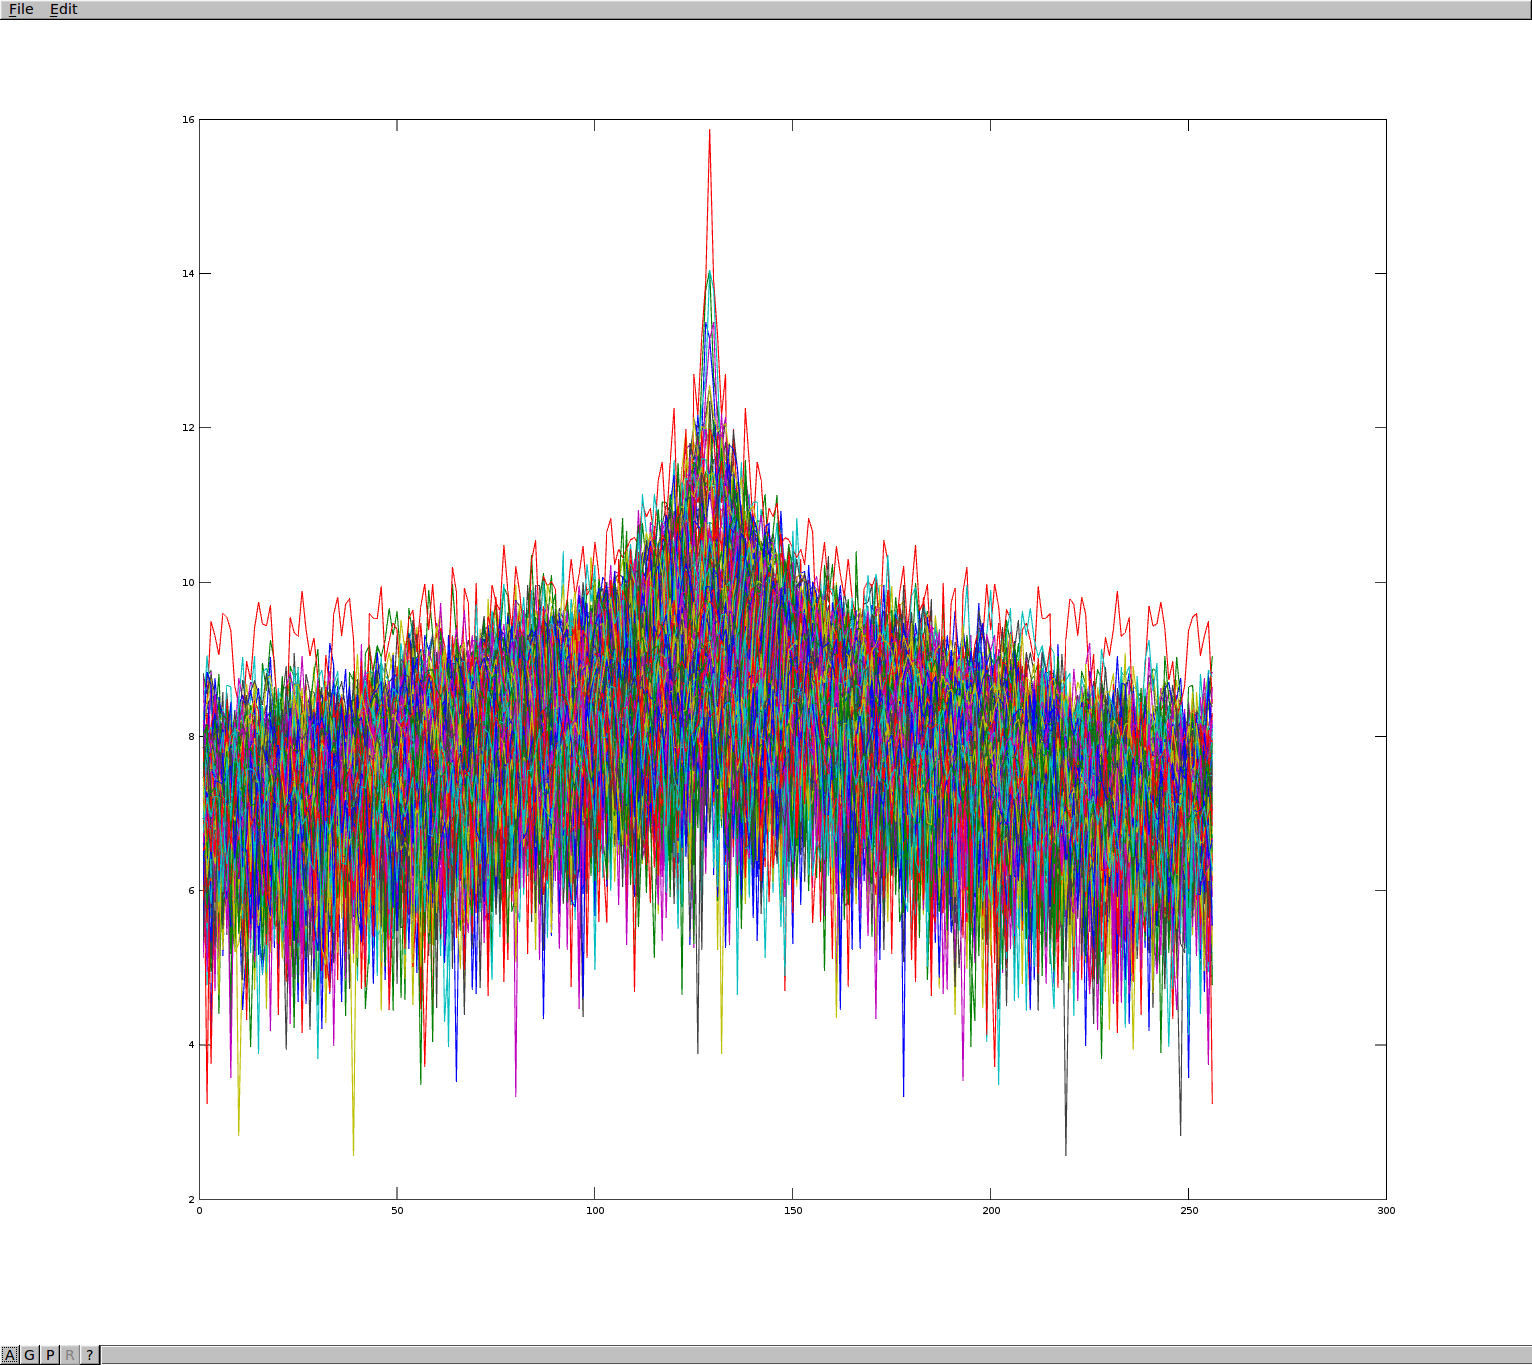
\includegraphics[width=\textwidth]{../code/3_out/bricks.png}
        \caption{FFT applied to bricks.png}
    \end{subfigure}

    \caption{Spectrum of the FFT for two different images.}
    \label{fig:3-1}
\end{figure}

The code used to generate the images presented in Figure~\ref{fig:3-1}.
\inputminted[linenos=true]{octave}{../code/3.1.m}
